\textbf{COLUNI 2019 -- Questão 35}\par\medskip Leia o texto abaixo do Discurso final do Filme “O Grande Ditador”, de Charles Chaplin, e observe a figura retirada do mesmo filme:

\par

\textbf{Discurso Final do Filme “O Grande Ditador”}

\par

Sinto muito, mas não pretendo ser um imperador. Não é esse o meu ofício. Não pretendo governar ou conquistar quem quer que seja. Gostaria de ajudar – se possível – judeus, o gentio... negros... brancos. Todos nós desejamos ajudar uns aos outros. Os seres humanos são assim. Desejamos viver para a felicidade do próximo – não para o seu infortúnio. Por que havemos de odiar e desprezar uns aos outros? Neste mundo há espaço para todos. A terra, que é boa e rica, pode prover a todas as nossas necessidades. O caminho da vida pode ser o da liberdade e da beleza, porém nos extraviamos. A cobiça envenenou a alma dos homens... levantou no mundo as muralhas do ódio... e tem-nos feito marchar a passo de ganso para a miséria e os morticínios. [...] Neste mesmo instante a minha voz chega a milhares de pessoas pelo mundo afora... milhões de desesperados, homens, mulheres, criancinhas... vítimas de um sistema que tortura seres humanos e encarcera inocentes. [...] Os homens que odeiam desaparecerão, os ditadores sucumbem e o poder que do povo arrebataram há de retornar ao povo. E assim, enquanto morrem homens, a liberdade nunca perecerá. [...] Não sois máquina! Homens é que sois! E com o amor da humanidade em vossas almas! Não odieis! Só odeiam os que não se fazem amar... os que não se fazem amar e os inumanos! Soldados! Não batalheis pela escravidão! Lutai pela liberdade! [...] Vós, o povo, tendes o poder de tornar esta vida livre e bela... de fazê-la uma aventura maravilhosa. Portanto – em nome da democracia – usemos desse poder, unamo-nos todos nós. Lutemos por um mundo novo... um mundo bom que a todos assegure o ensejo de trabalho, que dê futuro à mocidade e segurança à velhice. [...] Hannah, estás me ouvindo? Onde te encontrares, levanta os olhos! Vês, Hannah? O sol vai rompendo as nuvens que se dispersam! Estamos saindo da treva para a luz! Vamos entrando num mundo novo – um mundo melhor, em que os homens estarão acima da cobiça, do ódio e da brutalidade. Ergue os olhos, Hannah! A alma do homem ganhou asas e afinal começa a voar. Voa para o arco-íris, para a luz da esperança. Ergue os olhos, Hannah! Ergue os olhos! (Disponível em: <http://www.culturabrasil.org/discurso\_grande\_ditador\_chaplin.htm>. Acesso em: 2 out. 2018. Adaptado.)

\par

\textbf{Chaplin brinca com o globo terrestre em cena clássica de "O Grande Ditador"...}

% COLUNI-AUTO-FIGURES-BEGIN
\begin{figure}[htbp]
\centering
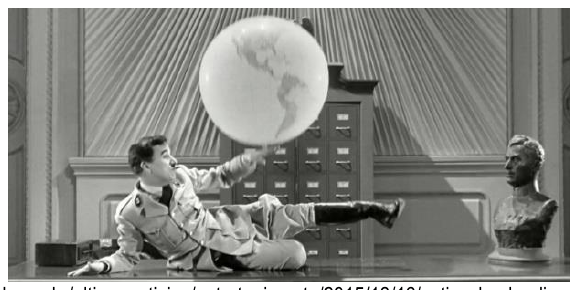
\includegraphics[width=0.95\linewidth]{static/simulados/coluni/figuras/2019/questao-35/figura-1.png}
\end{figure}
% COLUNI-AUTO-FIGURES-END

\par

(Disponível em: <https://noticias.bol.uol.com.br/ultimas-oticias/entretenimento/2015/12/16/satira-de-chaplin-ao-nazismo-de-hitler-o-grande-ditador- completa-75-anos.htm?cmpid=copiaecola>. Acesso em: 2 out. 2018.)

\par

O Filme "O Grande Ditador" foi lançado em 1940 durante a Segunda Guerra Mundial e faz uma sátira do regime do ditador da Alemanha, Adolf Hitler. Sobre o regime nazista da Alemanha, que levou à Segunda Guerra Mundial e a crítica feita por Chaplin em seu filme, assinale a afirmativa CORRETA:

\begin{enumerate}
\item Assim como está descrito no discurso final do filme, o regime nazista acreditava e defendia o sistema
        democrático como um poder do povo para buscar a felicidade.
\item Assim como está descrito no discurso final do filme, o regime nazista era pacifista e contrário à
        militarização, como é demonstrado no discurso de Chaplin.
\item Assim como está descrito no discurso final do filme, o regime nazista queria um mundo de fraternidade entre os
        povos, etnias e religiões; tal como visto na cena do filme na qual o personagem brinca com o Globo terrestre.
\item O discurso de "O Grande Ditador" faz um apelo ao respeito às diferenças entre os homens e defende a
        esperança de um mundo melhor para todos, ao contrário do que era defendido pelo regime nazista.\end{enumerate}
